\documentclass[12pt]{article}
\usepackage[utf8]{inputenc}
\usepackage{graphicx}
\usepackage{amsmath}
\usepackage{hyperref}
\usepackage{subcaption}
\usepackage{float}

\title{Modeling and Simulation of Earth's Average Global Temperature}
\author{Palmisano Luca \\ Bourgeois Noé}
\date{November 2023}

\begin{document}

\maketitle
\newpage

\section{Introduction}
The present report outlines the outcomes of a series of simulations designed to model the Earth's average global temperature. Using a range of models, from a basic Energy Balance Model (EBM) to more complex variations that integrate factors such as albedo and emissivity, this study aims to offer insights into the dynamics of Earth's climate system and the factors shaping its temperature.

\section{Methodology}
The results are obained by simulating Earth's temperature through a series of models. Starting with the Basic Energy Balance Model (EBM) and progressively expand to include additional factors such as variations in albedo and emissivity. 

For each model variation, the equilibrium temperature was computed whenever possible. Subsequently, simulations were conducted to observe the temperature's evolution over a span of 10,000 years. Leveraging the Octave software for numerical computations to solve the complex differential equations inherent in the models, the study then proceeded to analyze and discuss the obtained results, highlighting the differences between each model.

\section{Results}

\subsection{EBM: Equilibrium Temperature}
The equilibrium temperature of the system in the Energy Balance Model (EBM) is established by ensuring that the incoming solar radiation equals the outgoing longwave radiation\cite{kaper-2013-math-ac-equilibrium}.

\begin{equation} \label{eq:equilibrium-0}
    Q(1 - \alpha) = \sigma T^4
\end{equation}

\noindent The equation \ref{eq:equilibrium-0} can then be rearranged to isolate $T$:
\begin{equation} \label{eq:equilibrium-1}
    T = \left( \frac{Q(1 - \alpha)}{\sigma} \right)^{\frac{1}{4}}
\end{equation}

\noindent The values can then be substituted in \ref{eq:equilibrium-1}, which give us:
\begin{equation}
    T = \left( \frac{342 \times (1 - 0.3)}{5.67 \times 10^{-8}} \right)^{\frac{1}{4}} \approx 254.91 \, \text{K} \, ({-18.24}^\circ C)
\end{equation}

Comparing it to Earth's average temperature (${14.5}^\circ C$), we see a notable difference. This is because the model doesn't consider the \textit{greenhouse effect} and other factors affecting Earth's global temperature.

\begin{figure}[H]
    \centering
    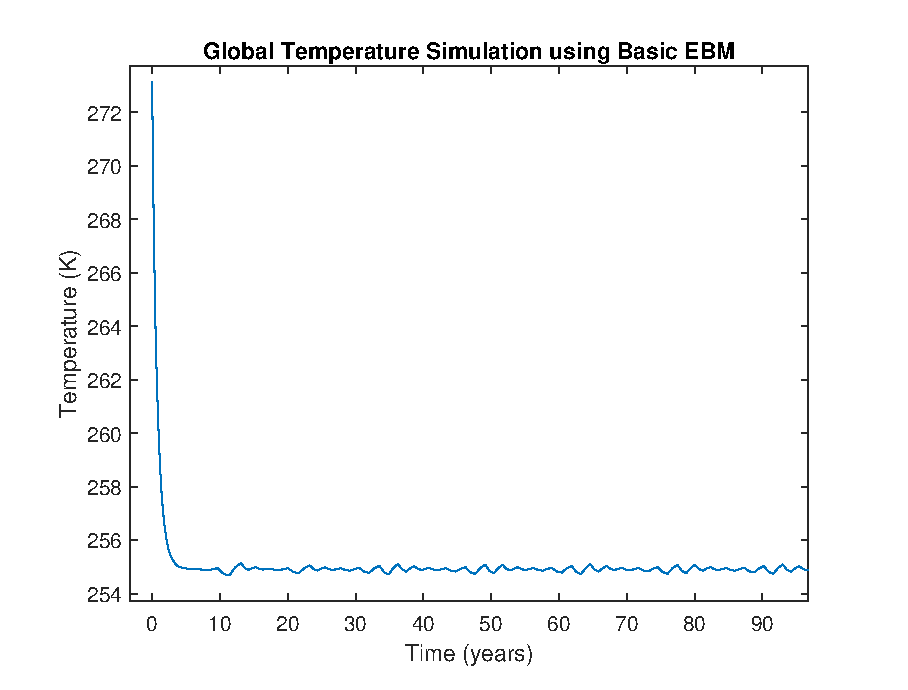
\includegraphics[width=0.7\textwidth]{images/ebm_basic.eps}
    \caption{Simulation of the basic EBM}
    \label{fig:basic_ebm}
\end{figure}

\subsection{EBM: Albedo variation}

The albedo of the Earth is not constant, and varies with the seasons. The albedo is higher in the winter due to the presence of snow and ice, and lower in the summer due to the presence of vegetation\cite{kaper-2013-math-ac-albedo}.

\begin{figure}[H]
    \centering
    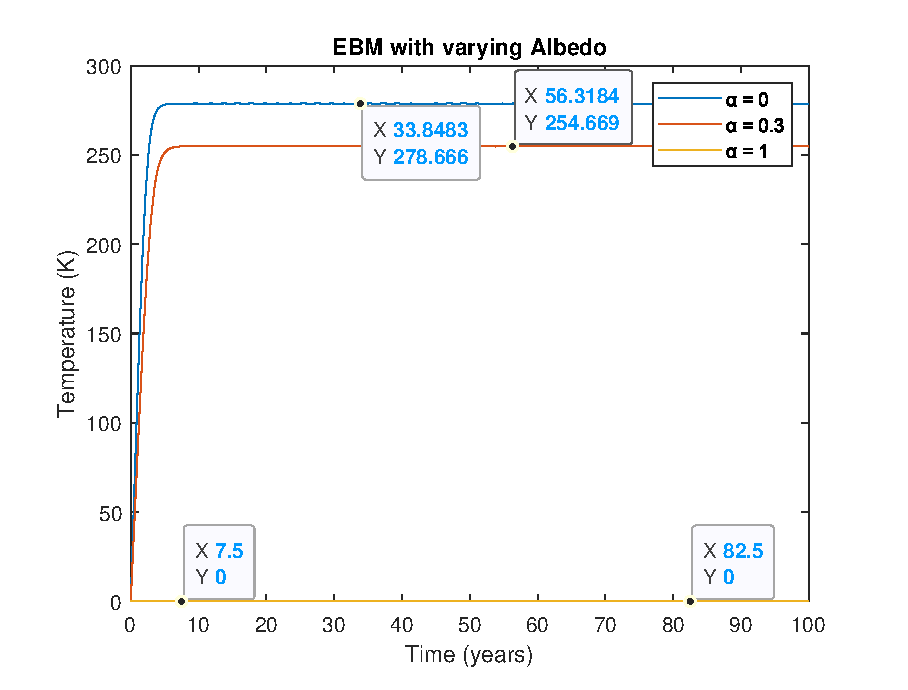
\includegraphics[width=0.7\textwidth]{images/albedo_extremes.eps}
    \caption{Simulation of the basic EBM with different albedos}
    \label{fig:albedo_extremes}
\end{figure}

For an albedo ($\alpha$) of 0, which mean complete absorption of incoming solar radiation, the equilibrium temperature is approximately 278.68 Kelvin. In contrast, with an albedo of 1, indicating total reflection of incoming solar radiation, the equilibrium temperature is always 0 Kelvin. 

These results highlight the significant impact of albedo on the Earth's temperature. An albedo of 1 represents an extreme and theoretical scenario where all incoming solar radiations are reflected, resulting in no energy absorption and a theoretical equilibrium temperature of absolute zero. In contrast, an albedo of 0 leads to higher temperatures due to the absorption of all incoming solar radiation.

\subsection{Emissivity Dependent OLR} \label{section:olr-emissivity}
The equilibrium temperature of the system, considering emissivity in the Energy Balance Model (EBM), is calculated by modifying the original equation\ref{eq:equilibrium-0} to include the emissivity factor\cite{kaper-2013-math-ac-emissivity}.

\begin{equation} \label{eq:emissivity-0}
    Q(1 - \alpha) = \epsilon\sigma T^4
\end{equation}

\noindent The equation \ref{eq:emissivity-0} can then be rearranged to isolate $T$:
\begin{equation} \label{eq:emissivity-1}
    T = \left( \frac{Q(1 - \alpha)}{\epsilon\sigma} \right)^{\frac{1}{4}}
\end{equation}

\noindent The values can then be substituted in \ref{eq:emissivity-1}, which give us:
\begin{equation}
    T = \left( \frac{342 \times (1 - 0.3)}{0.61 \times 5.67 \times 10^{-8}} \right)^{\frac{1}{4}} \approx 288.44 \, \text{K} \, ({15.29}^\circ C)
\end{equation}

This equilibrium temperature aligns more closely with the Earth's actual average surface temperature, highlighting the significant impact of emissivity in the energy balance model. In the case where the Earth does not emit any longwave radiation ($\epsilon=0$), there is a noticeable increase of almost 85 Kelvin per year. However, this particular case is not depicted in the figure \ref{fig:ebm_emissivity} to ensure a clear visualization of other results.

\begin{figure}[H]
    \centering
    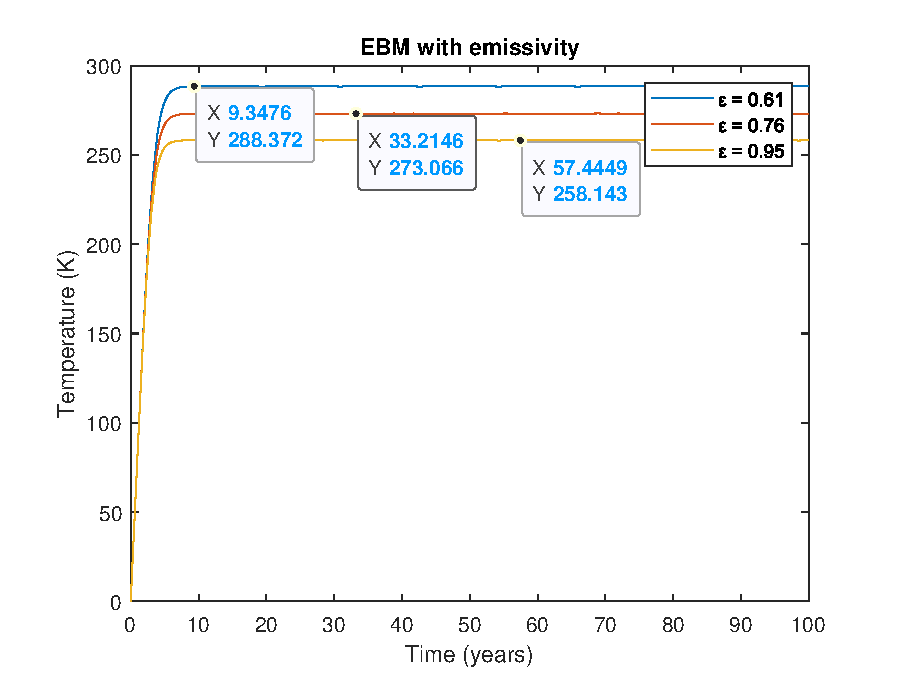
\includegraphics[width=0.7\textwidth]{images/ebm_emissivity_diff.eps}
    % \caption{Simulation of EBM with different emissivity factors}
    \caption{EBM simulation with typical $\epsilon=0.61$, $\epsilon=0.76$, showing negligible temperature change, and near maximum $\epsilon=0.95$, showing a small temperature decrease. This plot represents a more realistic scenario with a higher emissivity, resulting in minimal temperature variation over time.}
    \label{fig:ebm_emissivity}
\end{figure}

\subsection{Temperature Dependent OLR} \label{section:olr-temperature}
In this model, the Outgoing Longwave Radiation (OLR) is considered to be a function of temperature, represented by \( A + BT \), where \( A \) and \( B \) are constants. This approach acknowledges the fact that the Earth's radiation into space varies with its surface temperature\cite{kaper-2013-math-ac-budyko}.

% FIXME: Where does this comes from
% The equilibrium temperature under this model, represented by the equation \( R\frac{dT}{dt} = Q(1 - \alpha) - (A + BT) \), aligns more closely with empirical observations when compared to the basic EBM. This model also accounts for feedback mechanisms that are temperature-dependent offering a more nuanced understanding of the Earth's climate system.

\begin{figure}[H]
    \centering
    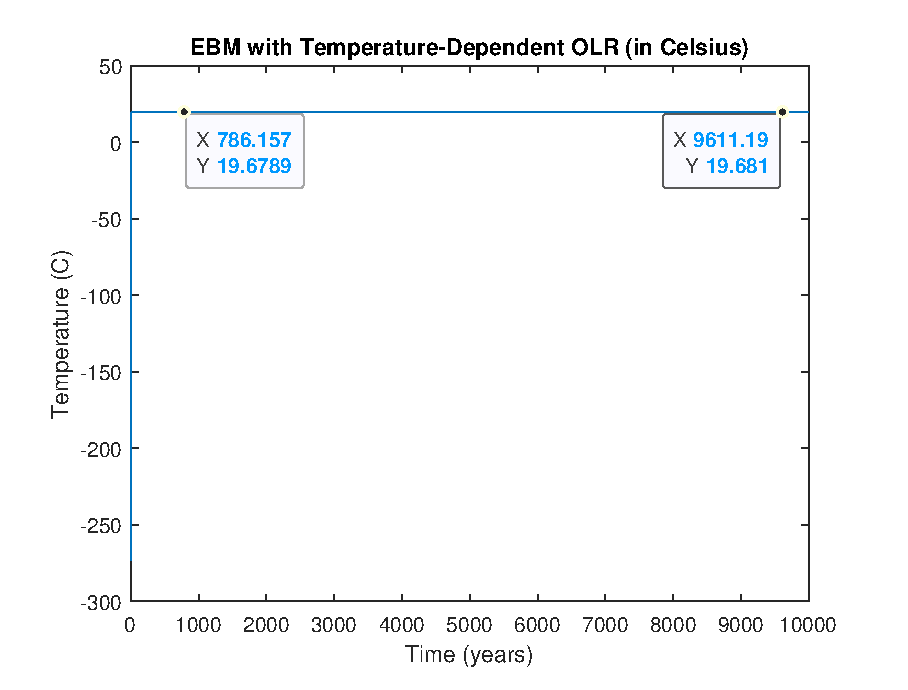
\includegraphics[width=0.7\textwidth]{images/temperature_dependent_olr.eps}
    \caption{Simulation of the EBM with temperature dependent OLR}
    \label{fig:ebm_temperature_olr}
\end{figure}

\subsection{Temperature Dependent Albedo} \label{section:albedo-temperature}
The model incorporating temperature-dependent albedo reflects the dynamic nature of the Earth's surface. As the temperature varies, so does the albedo, due to factors like melting ice and snow cover\cite{kaper-2013-math-ac-albedo}. In this model, elevated temperatures can cause a decrease in albedo, while a reduction in temperatures can lead to an increase in albedo.

\begin{figure}[H]
    \centering
    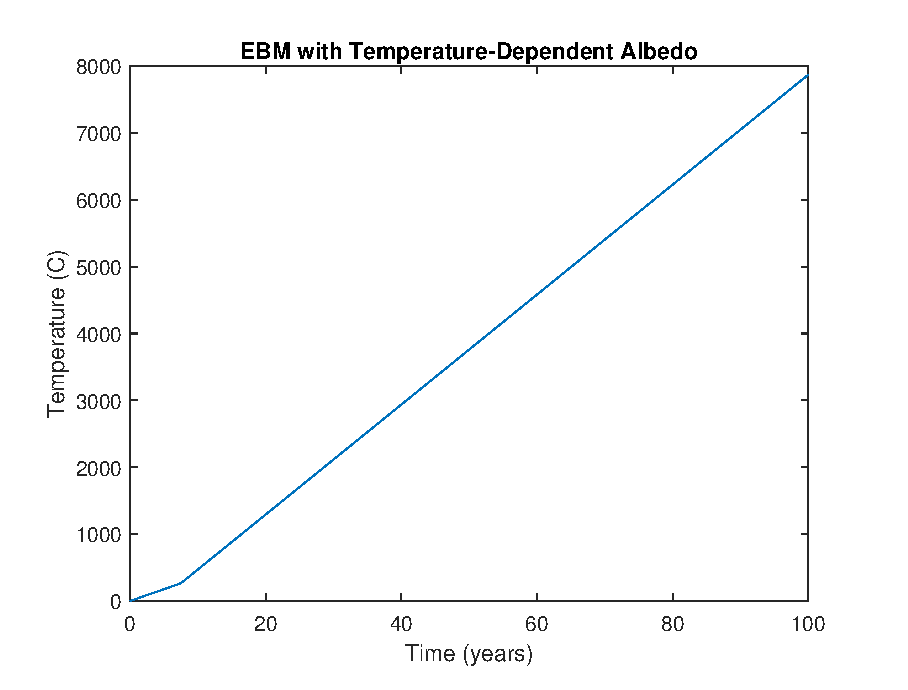
\includegraphics[width=0.7\textwidth]{images/temperature_dependent_albedo.eps}
    \caption{Simulation of the EBM with temperature-dependent albedo}
    \label{fig:ebm_temperature_albedo}
\end{figure}

\section{Discussion}
% Analyze the results you've presented.
% How do the models compare with each other?
% Discuss the implications of your findings, especially in the context of climate change.
% Are there any limitations or notable aspects of the models that affected the results?

\subsection{Emissivity and Temperature-Dependent Models}

The results from the simulations raise interesting points of discussion, particularly regarding the relative accuracy of the models in predicting Earth's average temperature. The model incorporating emissivity (\ref{section:olr-emissivity}) yielded a temperature closer to the real-world average of ${14.84}^\circ C$, whereas the temperature dependent OLR model (\ref{section:olr-temperature}) deviated more significantly from this value.

\subsubsection{Impact of Emissivity in Climate Models}
The inclusion of emissivity in the energy balance model significantly enhances its realism. Emissivity, representing the Earth's ability to emit radiation, is a key factor in the Earth's energy balance. Our simulation using an emissivity factor close to Earth's real value ($\approx 0.61$) resulted in a temperature estimation that aligns more closely with the actual average global temperature. This highlights the importance of emissivity in modeling Earth's climate and suggests that it captures essential aspects of the Earth's radiation dynamics.

\subsubsection{Challenges with Temperature-Dependent OLR}
The model with temperature dependent OLR, despite adding complexity, may not have been as effective in mimicking the actual climate system. The parameters \( A \) and \( B \) in the \( A + BT \) formulation of OLR are crucial. If these parameters do not accurately reflect the Earth's real radiation properties, the model's predictions can deviate from real-world temperatures. This indicates the challenge of accurately calibrating climate models to match the complexities of the Earth's climate system.

\subsection{Model Limitations and Realism}
Both models are simplified representations of the actual climate system. The differences in their predictions highlight the impact of various climatic factors on Earth's temperature. It also emphasizes the need for precise parameter selection and calibration in climate modeling. The closer alignment of the emissivity model with the actual average temperature suggests that, for our models, the emissivity factor is more crucial in capturing the key aspects of Earth's thermal radiation balance compared to the linear relationship of temperature dependent OLR.

\section{Conclusion}
% Summarize your main findings.
% Reflect on what these results mean for our understanding of Earth's climate system.
Comparing the two models shows how tricky climate modeling can be. It emphasizes the importance of accurately choosing and adjusting model details to reflect the complexities of the real-world climate system. A notable instance is the model where the Outgoing Longwave Radiation (OLR) depends on the temperature, which, in turn, is influenced by satellite observations. If these values are not precise, it can significantly impact the results.

\newpage
\bibliographystyle{unsrt}
\bibliography{bibliography}

\end{document}
